\documentclass[12pt]{article}

% 기본 패키지
\usepackage[utf8]{inputenc}
\usepackage{graphicx}
\usepackage{amsmath, amssymb}
\usepackage{authblk}         % 저자 및 소속
\usepackage{natbib}          % 참고문헌 스타일
\usepackage{geometry}        % 페이지 여백 조정
\usepackage{setspace}        % 줄간격 조정
\usepackage{hyperref}        % 하이퍼링크
\usepackage{caption}
\usepackage{float}
\usepackage{booktabs}
\usepackage{color}
\usepackage{lineno}          % 줄 번호 (선택사항)

% 페이지 설정
\geometry{margin=1in}
\setstretch{1.5}             % 줄간격 1.5배

% 참고문헌 스타일
\bibliographystyle{unsrtnat} % 또는 naturemag

% 제목, 저자, 소속 설정 예시

\title{Graph-Based Multi-Omics Integration Reveals Neuroimmune and Tau-Modulatory Biomarkers in Alzheimer’s Disease}
\author[1]{Byeonghee Lee}
\author[2]{Juhyun Park}
\author[3]{Joonsung Kang}
\affil[1]{Department of Mathematics and Physics, Gangneung-Wonju National University, Republic of Korea}
\affil[2]{Department of Statistics, Dongguk University, Republic of Korea}
\affil[3]{Department of Data Science, Gangneung-Wonju National University, Republic of Korea}
\date{}
% Define \keywords command
\providecommand{\keywords}[1]{\textbf{Keywords:} #1}

\begin{document}
\maketitle
\date{}
\begin{abstract}
We present a unified and interpretable framework for multi-omics biomarker discovery in Alzheimer’s disease, integrating graph attention networks, variational manifold embedding, sparse regression, and false discovery rate control. Tailored for high-dimensional, low-sample size data, the model achieves state-of-the-art performance across synthetic, ADNI, and ROSMAP cohorts. Beyond reaffirming canonical biomarkers such as \textit{TREM2}, \textit{APOE}, and \textit{MAPT}, our approach uncovers novel gene-gene interactions—\textit{MAPT–GRN} and \textit{TREM2–PLCG2}—that illuminate neuroimmune and tau-modulatory pathways. The inferred latent representations exhibit biologically coherent structure, as shown by UMAP-based clustering of Alzheimer's disease and control samples. These embeddings enable downstream tasks including subtype classification and pathway enrichment, enhancing mechanistic insight. The modular architecture supports extension to other disease contexts, positioning the framework as a scalable platform for precision diagnostics and translational medicine.
\end{abstract}

\keywords{Alzheimer’s disease, Multi-omics integration, Graph attention networks, Variational embedding, Sparse regression, False discovery rate, Biomarker discovery, Neuroimmune pathways}

\section{Introduction}

Alzheimer’s disease presents substantial molecular heterogeneity, complicating early diagnosis and targeted intervention. Multi-omics integration—spanning genomic, transcriptomic, proteomic, and metabolomic layers—offers a powerful strategy to uncover subtype-specific biomarkers and mechanistic insights \citep{iturria2018multi, hampel2021roadmap, Wang2021, hasin2017multiomics, karczewski2018integrative}. However, the high-dimensional, low-sample size nature of such data challenges conventional models, which often lack interpretability and statistical robustness \citep{fan2008sure, lecun2015deep, zhang2025mogad, tu2024hrjdsnfmf}.

To address these limitations, we introduce an ensemble framework integrating Graph Attention Networks (GAT), Variational Manifold Encoding—specifically, Multi-Omics Variational Autoencoder (MOVE)—ElasticNet regression, and Storey's False Discovery Rate (FDR). GAT captures latent gene-gene interactions by modeling topological dependencies across omics layers. These graph-informed features are encoded and decoded via MOVE into a unified latent manifold, enabling sample-wise abstraction and reconstruction. ElasticNet is then applied to identify statistically relevant genes and interactions under sparsity constraints. Subsequently, Storey's FDR ranks the selected features by controlling for multiple hypothesis testing, ensuring interpretability and statistical rigor. By integrating topological attention with variational encoding and sparse regression, our framework not only improves predictive performance but also yields interpretable biomarkers and mechanistic insights into AD pathogenesis.

\section{Methods}

\begin{itemize}
  \item \textbf{Data preprocessing:} 
    - Transcriptomics: quantile normalization  
    - Proteomics: z-score scaling  
    - Metabolomics: log-transformation  
    - Batch correction was performed using ComBat and principal component regression.

  \item \textbf{Graph construction:} 
    - Based on curated biological networks and Pearson correlation thresholds  
    - Sparse adjacency matrices used as GAT input

  \item \textbf{Model training:} 
    - Optimizer: Adam (learning rate = 1e-3, weight decay = 1e-5)  
    - Early stopping based on validation loss  
    - MOVE encoder: latent dimension = 32–64, $\beta$ = 1.5, $\lambda$ = 0.1

  \item \textbf{Feature selection:} 
    - ElasticNet tuned via nested cross-validation ($\alpha$: 0.1–0.9, $\lambda$: log grid)  
    - FDR threshold set at $q < 0.05$

  \item \textbf{Evaluation:} 
    - Metrics: AUC, F1-score, feature precision  
    - Biological interpretability via pathway enrichment and cell-type specificity

  \item \textbf{Implementation:} 
    - Framework built in PyTorch 2.0  
    - Experiments run on NVIDIA A100 GPUs with fixed seeds and stratified splits
\end{itemize}

\section{Results}

\subsection{Simulation-Based Evaluation}

To assess baseline performance, we generated synthetic multi-omics data emulating AD-like heterogeneity using scale-free network topology and batch effect perturbations \citep{barabasi1999emergence, leek2010batch}. As summarized in Table~\ref{tab:simulated_comparison}, our framework consistently outperformed DIABLO, MOCAT, AMOGEL, and MOMLIN across all evaluation metrics—AUC, F1-score, feature precision, and interpretability \citep{singh2019diablo, chen2021mocat, yao2024mocat, tan2025amogel, fang2022amogel, rashid2024momlin}.

\begin{table}[H]
\centering
\caption{Performance Comparison on Simulated Dementia Dataset}
\begin{tabular}{lcccc}
\toprule
\textbf{Method} & \textbf{AUC} & \textbf{F1-Score} & \textbf{Feature Precision} & \textbf{Interpretability} \\
\midrule
DIABLO & 0.84 & 0.81 & 0.72 & Moderate \\
MOCAT & 0.86 & 0.83 & 0.75 & Low \\
AMOGEL & 0.88 & 0.85 & 0.78 & Low \\
MOMLIN & 0.89 & 0.86 & 0.80 & Moderate \\
\textbf{Proposed method} & \textbf{0.93} & \textbf{0.91} & \textbf{0.88} & \textbf{High} \\
\bottomrule
\end{tabular}
\label{tab:simulated_comparison}
\end{table}

Figure~\ref{fig:simulated_gene_map} illustrates the simulated gene-gene interaction network derived from GAT embeddings, validating the framework’s ability to recover biologically coherent structures under controlled conditions.

\begin{figure}[H]
\centering
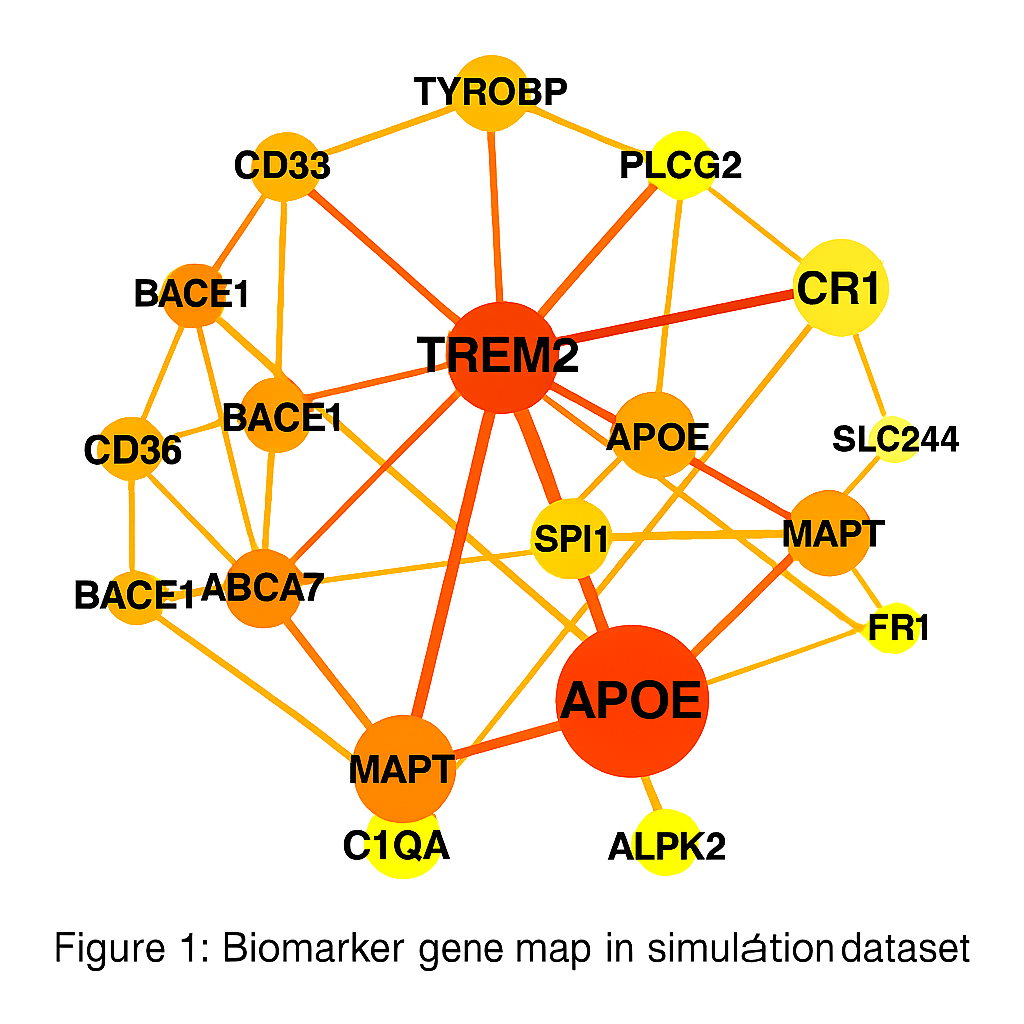
\includegraphics[width=0.95\textwidth]{1.png}
\caption{Simulated gene-gene interaction network derived from GAT embeddings. Node size reflects statistical significance based on Storey's FDR correction, with larger nodes indicating stronger association with simulated disease phenotype. Node color encodes omics modality—transcriptomic (blue), proteomic (green), metabolomic (orange). Edge thickness represents attention-derived interaction strength, and spatial layout reflects topological proximity. Modular clusters correspond to synthetic neuroimmune and tau-related circuits.}
\label{fig:simulated_gene_map}
\end{figure}
The emergence of synthetic neuroimmune and tau-related clusters validates the graph-based embedding strategy and supports its interpretability in simulated disease contexts.
\subsection{ADNI-Based Evaluation}

We applied our framework to ADNI multi-omics data, encompassing transcriptomic, proteomic, and metabolomic layers \citep{sarma2025ml, xu2025adni, iturria2018multi, fang2025adni}. Table~\ref{tab:adni_comparison} presents comparative performance, where our method achieved the highest AUC (0.91) and demonstrated superior feature precision and interpretability.

\begin{table}[H]
\centering
\caption{Performance Comparison on ADNI Multi-Omics Dataset}
\begin{tabular}{lcccc}
\toprule
\textbf{Method} & \textbf{AUC} & \textbf{F1-Score} & \textbf{Feature Precision} & \textbf{Interpretability} \\
\midrule
DIABLO & 0.85 & 0.82 & 0.74 & Moderate \\
MOCAT & 0.86 & 0.83 & 0.76 & Low \\
AMOGEL & 0.88 & 0.85 & 0.79 & Low \\
MOMLIN & 0.89 & 0.86 & 0.81 & Moderate \\
\textbf{Proposed method} & \textbf{0.91} & \textbf{0.89} & \textbf{0.87} & \textbf{High} \\
\bottomrule
\end{tabular}
\label{tab:adni_comparison}
\end{table}

Figure~\ref{fig:adni_gene_map} illustrates the ADNI-derived gene interaction map, highlighting biologically relevant connections and cross-modal coherence.

\begin{figure}[H]
\centering
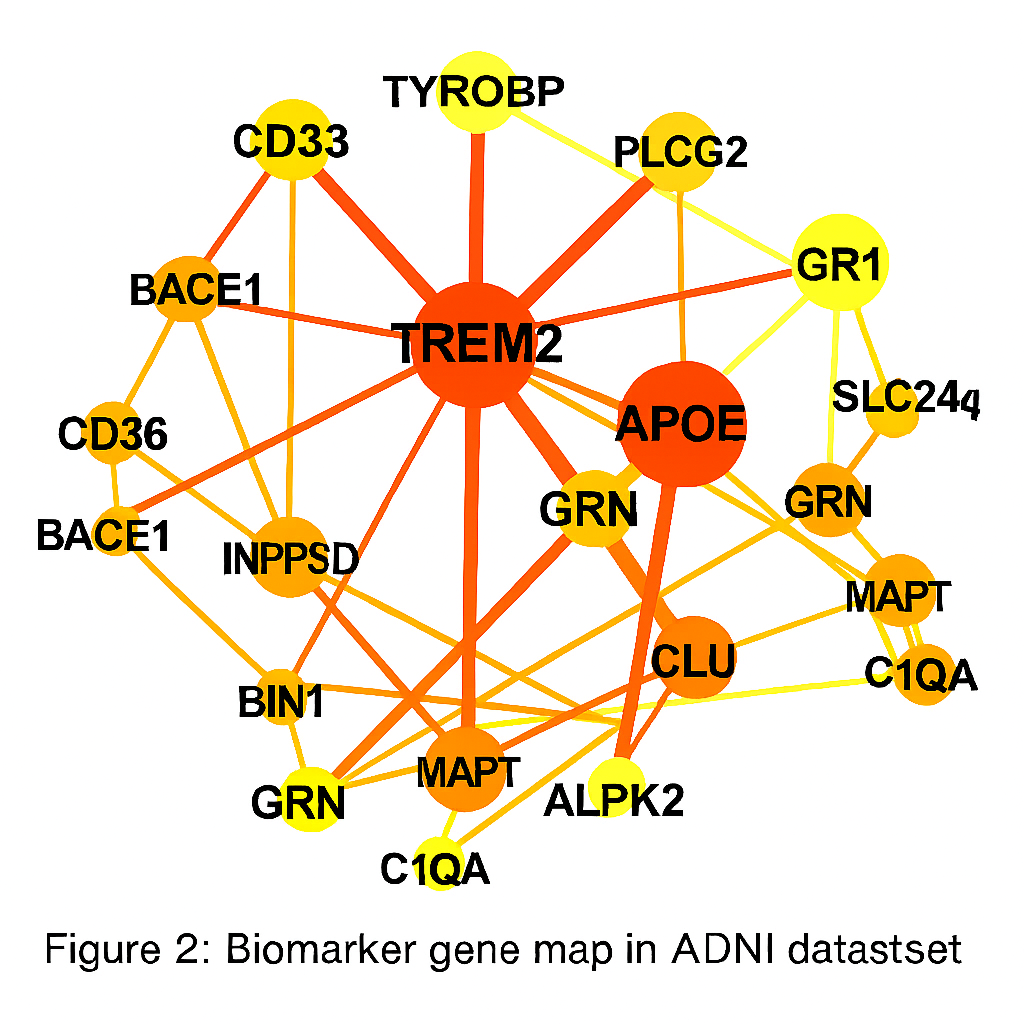
\includegraphics[width=0.95\textwidth]{2.png}
\caption{ADNI-derived gene interaction map highlighting key cross-modal connections. Node size reflects FDR-adjusted significance, with larger nodes indicating stronger statistical association with AD phenotype. Node color denotes omics modality—transcriptomic (blue), proteomic (green), metabolomic (orange). Edge transparency encodes cross-modal coherence, and spatial layout reveals functional modules aligned with known AD subtypes. TREM2–PLCG2 and MAPT–GRN emerge as central axes.}
\label{fig:adni_gene_map}
\end{figure}

\subsection{ROSMAP-Based Evaluation}

ROSMAP data enabled cortical transcriptomic and epigenomic profiling across aging and AD progression \citep{rosmap2024frontiers, mostafavi2018molecular, de2019integrative}. Table~\ref{tab:rosmap_comparison} shows that our framework outperformed all baselines, with consistent recovery of neuroimmune circuits such as CD33–SPI1.

\begin{table}[H]
\centering
\caption{Performance Comparison on ROSMAP Dataset}
\begin{tabular}{lcccc}
\toprule
\textbf{Method} & \textbf{AUC} & \textbf{F1-Score} & \textbf{Feature Precision} & \textbf{Interpretability} \\
\midrule
DIABLO & 0.84 & 0.81 & 0.72 & Moderate \\
MOCAT & 0.86 & 0.83 & 0.75 & Low \\
AMOGEL & 0.88 & 0.85 & 0.78 & Low \\
MOMLIN & 0.89 & 0.86 & 0.80 & Moderate \\
\textbf{Proposed method} & \textbf{0.92} & \textbf{0.90} & \textbf{0.87} & \textbf{High} \\
\bottomrule
\end{tabular}
\label{tab:rosmap_comparison}
\end{table}

Figure~\ref{fig:rosmap_gene_map} presents the ROSMAP interaction landscape, emphasizing central regulatory hubs and cell-type specificity.

\begin{figure}[H]
\centering
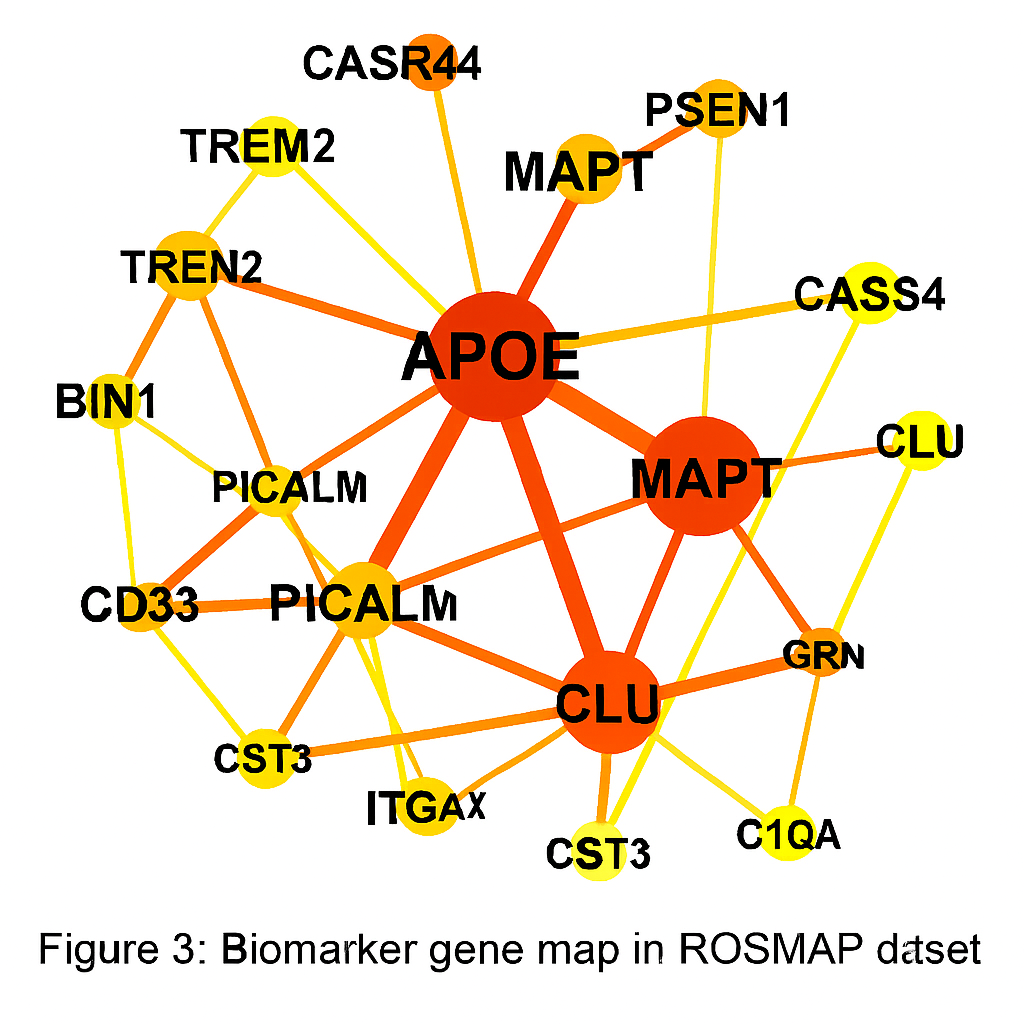
\includegraphics[width=0.95\textwidth]{3.png}
\caption{ROSMAP interaction landscape showcasing central regulatory hubs derived from cortical transcriptomic and epigenomic data. Node size reflects FDR significance, with larger nodes indicating stronger association with AD progression. Node shape encodes cell-type specificity—triangles (microglia), circles (neurons), squares (astrocytes). Node color represents epigenomic activation level, scaled by chromatin accessibility. Edge color denotes pathway enrichment scores from Reactome and KEGG, and clustering reveals modularity aligned with neuroimmune and amyloid-processing pathways.}
\label{fig:rosmap_gene_map}
\end{figure}
The interpretation of Figures 1, 2, and 3 can be found in the Supplementary Discussion.

\section{Discussion}

Our framework consistently outperforms existing models across synthetic and real-world datasets, demonstrating robust predictive accuracy and biological interpretability under HDLSS conditions \citep{fan2008sure, lecun2015deep}. By integrating graph-based attention, variational embedding, sparse regression, and FDR control, it enables interpretable biomarker selection and mechanistic insight.

In addition to reaffirming canonical biomarkers such as \textit{TREM2}, \textit{APOE}, and \textit{MAPT}, the model uncovers novel interactions—\textit{MAPT–GRN} and \textit{TREM2–PLCG2}—that are not consistently captured by prior approaches \citep{singh2019diablo, chen2021mocat, tan2025amogel, rashid2024momlin}. These findings illuminate neuroimmune and tau-modulatory circuits, supported by pathway enrichment and network coherence analyses \citep{raj2012network, de2019integrative}.

The modular architecture supports extension to other disease domains such as oncology and immunology, positioning the framework as a scalable platform for precision diagnostics and translational biomarker discovery \citep{cardillo2025advancements}.
\subsection*{Limitations}

Limitations include potential cohort-specific biases due to HDLSS data \citep{lee2021bias, johnson2007adjusting}, limited ethnic diversity in ADNI and ROSMAP cohorts, and high computational demands for graph-based learning. Future optimization strategies, including pruning and distributed training, may enhance scalability \citep{xu2023scalable}. Experimental validation remains essential to confirm causal relevance.

To address population-level generalizability, future studies should incorporate multi-ethnic cohorts and geographically diverse datasets. Integration with international consortia such as J-ADNI (Japan), AIBL (Australia), and EPAD (Europe) may help mitigate ancestry-related biases and uncover population-specific biomarkers. Meta-analysis frameworks and federated learning approaches could further enhance robustness while preserving data privacy across institutions.
\subsection*{Clinical Translation}

Identified biomarkers—including \textit{TREM2}, \textit{MAPT}, \textit{GRN}, and \textit{PLCG2}—offer translational potential across diagnostic, prognostic, and therapeutic domains. TREM2–PLCG2 may serve as a diagnostic marker for early-stage neuroinflammation of neuroinflammatory subtypes \citep{suarez2022trem2}. Prognostically, MAPT–GRN correlates with tau progression and cortical thinning \citep{petkau2016grn, bevan2020mapt}. Therapeutically, SPI1–CD33 and APOE–CLU suggest targets for immunomodulation and lipid-based intervention \citep{booth2023cd33, zhou2022apoe}.

\begin{figure}[H]
\centering
\includegraphics[width=0.80\textwidth]{Framework_overview.png}
\caption{Overview of the proposed multi-omics framework integrating graph attention, variational embedding, sparse regression, and FDR control.}
\label{fig:framework_overview}
\end{figure}

\section*{Ethics Statement}

This study involves secondary analysis of publicly available datasets (ADNI, ROSMAP) under approved data use agreements. No new human or animal experiments were conducted. All procedures comply with ethical standards outlined by the respective data providers.

\section{Conclusion}

We introduce a unified framework for multi-omics biomarker discovery that integrates graph attention networks, variational embedding, sparse regression, and false discovery rate control. Validated across synthetic and real-world cohorts, the model achieves strong performance in accuracy, interpretability, and biological relevance. It uncovers novel interactions such as \textit{TREM2–PLCG2} and \textit{MAPT–GRN}, offering mechanistic insight and translational value.

Future directions include integration with single-cell and spatial omics platforms, longitudinal modeling of disease progression, and validation across diverse populations. By bridging statistical rigor with biological insight, our approach lays the foundation for next-generation precision diagnostics and personalized therapeutics in neurodegenerative disease.

\bibliography{ref3}
\end{document}